\section{Isogenies, graphs, fibres, conductors, and transfer}\label{sec:isogenies}

The isogeny work is not a single failed shortcut. It contains several
different objects: explicit walks and map certificates, conductor and
endomorphism-ring calculations, fibre-aware bases, gluing and
higher-genus constructions, weak-node searches, graph-wide experiments,
and cryptographic scheme prototypes. Their obligations differ.

\subsection{What transport conserves}

For a homomorphism $\varphi:E(\F_q)\to E'(\F_q)$, let
$\kappa=\ker\varphi\cap E(\F_q)$. Suppose
$\B'\subset\varphi(E(\F_q))$ and take the complete rational pullback
$\B=\varphi^{-1}(\B')\cap E(\F_q)$. The recorded transport argument
states that the number of ordered $m$-decompositions of $R$ over $\B$
is $|\kappa|^{m-1}$ times the number of decompositions of $\varphi(R)$
over $\B'$. Each image tuple has $|\kappa|^m$ lifts, and exactly
$|\kappa|^{m-1}$ have the required sum.\src{TRANSFER}

This is a useful scoped statement. It applies to the declared
homomorphism and complete pullback domain. It does not prove that every
alternative factor-base geometry has the same cost, nor that every
non-homomorphic or higher-dimensional reduction is impossible. It
directs attention to three things that can still change: rational
kernel symmetry, destination geometry, and arithmetic/solver cost.
Map evaluation and source recovery remain additional costs.

Isogeny loops act as endomorphisms; on a fixed prime cyclic subgroup an
applicable endomorphism acts by a scalar. Faster evaluation can help
known-scalar multiplication or a generic walk. Turning it into a
non-generic unknown-log advantage requires another mechanism. The
portfolio correctly keeps these claims distinct in its newer transfer
and curve-identity rules.\src{FIBRES}\src{C-RULES}

\subsection{Conductor gaps and fibre-aware IC}

The conductor-gap programme examines whether endomorphism-ring levels
change the measured difficulty of a decomposition method. Two fixed CM
pairs with large prime gaps give recorded floor/crater counted-$S$
ratios 0.975 with 99\% interval [0.603,1.451] and 1.127 with interval
[0.922,1.342], across 192 verified records and 96 stored exact replays.
These observations do not resolve the general conductor-gap question;
they fail to detect an effect in those exact comparisons. Both sides'
unpriced work remains relevant.\src{CONDUCTOR}

Fibre closure and two-torsion symmetrisation can reduce redundant algebra
on a matched abscissa base. A later correction shows why the domain
must be specified: at matched column count, an apparent symmetry saving
can disappear. Similarly, the fibre-aware scaling panels improve a
specific method but show its IC/rho envelope widening with size at
fixed cofactor. The reported ratios rise roughly from 8--9 to 35--37
at cofactor four, and from 13--20 to 60--63 at cofactor 72.
\src{FIBRE-SCALE}\src{PRIOR}

The right question is therefore a controlled comparison on the same
transported target, base convention, subgroup and resource envelope.
Comparing two curves with different subgroup sizes or comparing an
orbit-redundant base to an already-quotiented base does not isolate
intrinsic hardness.

\subsection{The graph-building capability and its measured coverage}

The full-volcano work builds explicit finite graphs and routes, exports
explorers, verifies kernel maps, assigns conductor strata, and runs
bounded IC and generic solvers on selected vertices. This is a
substantial implemented capability. Graph generation, graph completeness
for a declared edge set, and graph-wide attack execution are three
different completion claims.\src{VOLCANO}

The accessible checkpoint covers three smaller classes with 24,823
declared vertices and 51 strata. The repaired checkpoint has 2,935
audited vertices: 989 in the mixed-conductor graph, 970 in the
three-power graph, and 976 in the two-power graph. All 51 strata have
samples. This is about 11.8\% of the declared vertex population,
not a completed graph-wide measurement.

\begin{table}[htbp]\small
\caption{Outcomes in the downloaded repaired checkpoint. They are
attempts across multiple arms and two target workloads per selected
vertex, not 46,960 independent curves. Source: \src{VOL-ARCHIVE}.}
\begin{tabular}{@{}lr@{}}\toprule
Quantity & Recorded count \\\midrule
Audited vertices / declared graph vertices & 2,935 / 24,823 \\
Strata sampled & 51 / 51 \\
Attempt records & 46,960 \\
Verified recoveries & 30,270 \\
Exhausted budgets & 14,626 \\
Timeouts & 2,064 \\
Relations found & 1,530,557 \\
Source relation trials & 74,829,850 \\
Actual decomposition calls & 71,296,000 \\
\bottomrule
\end{tabular}
\end{table}

Source trials and oracle calls differ because repeated queries can be
skipped before invoking the oracle. Timeout counters are unknown where
not emitted; they are not zero. Earlier report versions labelled source
trials as decompositions, and the corrected summary exposes both
denominators. Those corrections are a practical example of why raw
records and versioned summaries matter.

\begin{figure}[htbp]
\centering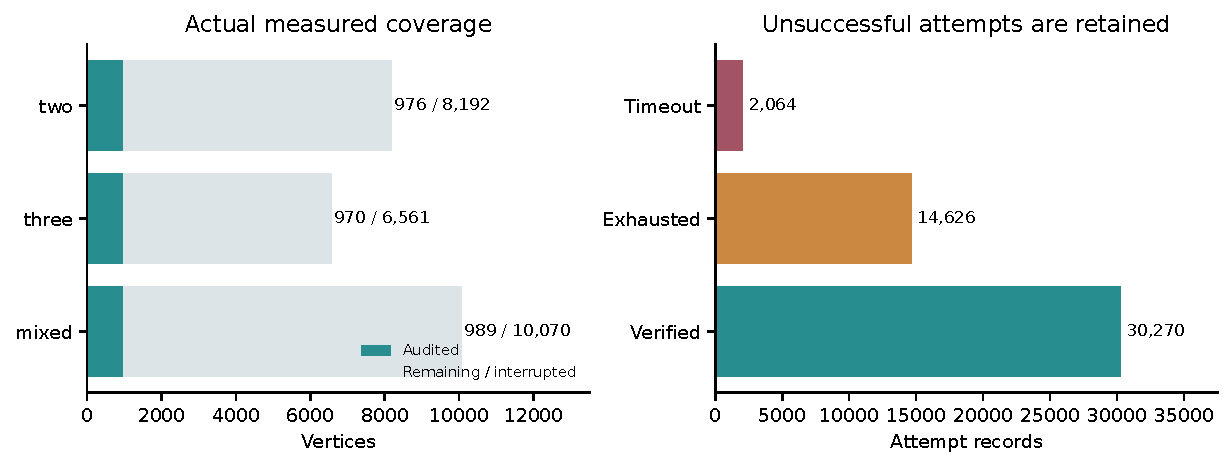
\includegraphics[width=\linewidth]{figures/volcano-coverage.pdf}
\caption{Coverage and outcomes of the actual 2,935-vertex checkpoint.
The left panel compares audited with remaining vertices in each of the
three finite graphs; the right panel preserves unsuccessful attempts.
This is a coverage chart, not an inference that unsampled vertices share
the same outcomes. All 51 strata are sampled. Source: \src{VOL-ARCHIVE}.}
\end{figure}

The three source models have very different largest prime subgroups:
61,751; 19,768,889,568,671; and 4,253. Their roughly 57--59-bit field
sizes must not be used as common subgroup security sizes. The original
A--E ambitions are much larger---about 7.83 billion expected vertices
and 515 strata---and remain separate incomplete work. The smaller
checkpoint cannot be described as completing those populations.

This review downloaded the archive and checked every one of its 29,409
manifest entries, with no missing entry or hash mismatch. That proves
byte consistency of this delivery. The checkpoint's solver audits are
same-implementation replays, not new independent validation by this
review. Its unqualified wall times and incomplete operation counts do
not establish a fastest-method or asymptotic claim.

\subsection{GHS mechanisms and the scope of a trapdoor demonstration}

The pinned main branch of \texttt{ghs-trapdoor} is a scaffold, but another
captured branch contains a Sage mechanism prototype. It describes a
composite-degree binary field $\F_{2^{20}}$ over $\F_{2^5}$, a weak curve,
an Artin--Schreier tower, a genus-four model, an explicit transfer, and a
small protected subgroup of order 7,717. The branch reports
homomorphism and subgroup-order checks, isogeny pullback, and end-to-end
toy ElGamal recovery.\src{GHS-MAIN}\src{GHS-BRANCH}

Those are mechanism claims on the branch, not a demonstrated scalable
escrow system. The toy destination solver is BSGS, whose square-root
cost is comparable to source rho at that tiny subgroup order. The
general claim that the public curve forces outsiders to use rho, or
that a secret chain is hard to replace with any useful public route,
requires additional analysis. Working-field ambiguity in the README's
Jacobian description also needs checking against the actual code and
certificates before a stronger transport claim is made. No fresh Sage
or Lean replay was performed here.

The distinction is especially important for ECC2K-130, whose extension
degree 131 is prime. A construction exploiting a degree-four extension
cannot simply be scaled by changing that parameter. The ten-lead
register contains finite order and map-class obstructions for particular
candidate Jacobians, but leaves other destinations and constructions
open.\src{TEN}

\subsection{What remains of the structural and hidden-route leads}

The structural-completeness draft organises seven families of known
isogeny/CM mechanisms. Its own correction now describes case-analysis
proof sketches that have not received independent review; an earlier
unconditional-proof sentence was removed. This paper therefore treats
it as an organised argument and source catalogue, not a proof that every
prime-field attack route has been exhausted.\src{STRUCTURAL}

A hypothetical hidden route should be assessed through separate
questions: mathematical existence, explicit construction, public
discoverability, subgroup action, destination advantage, evaluation and
recovery costs, and the availability of an equivalent public shortcut.
No inference about secret agency capability follows merely from a
large degree or a sparse weak class. Conversely, failing to make a
route practical in a toy study is not a proof of its universal
impossibility. These are the appropriate remaining obligations of the
programme's speculative endomorphism and isogeny leads.
